% This is samplepaper.tex, a sample chapter demonstrating the
% LLNCS macro package for Springer Computer Science proceedings;
% Version 2.20 of 2017/10/04
%
\documentclass[runningheads]{llncs}
%
\makeatletter
\usepackage[algoruled,boxed,lined]{algorithm2e}
\makeatletter
\g@addto@macro{\@algocf@init}{\SetKwInOut{Parameter}{Parameters}}
\makeatother
\usepackage{amsmath}
\usepackage{amssymb}
\usepackage{graphicx}

% Used for displaying a sample figure. If possible, figure files should
% be included in EPS format.
%
% If you use the hyperref package, please uncomment the following line
% to display URLs in blue roman font according to Springer's eBook style:
% \renewcommand\UrlFont{\color{blue}\rmfamily}
\usepackage{tikz}
\usetikzlibrary{trees}
\usetikzlibrary{automata, positioning}
\usepackage{listings}
\lstset{basicstyle=\ttfamily}
\usepackage{tcolorbox}
\usepackage{framed}
\usepackage{forest}
\usepackage{xcolor}
\usepackage{blkarray}
\usepackage{comment}
\usepackage{footnote}


\renewcommand{\Coloneqq}{\mathrel{\mathop{::}}=}

\lstdefinestyle{lstStyle}{
    language=C++,
    basicstyle=\small\ttfamily,
    tabsize=4,
    breaklines=true,
    showtabs=false,
    showspaces=false,
    showstringspaces=false,
    columns=flexible
}

\begin{document}
%
    \title{syntaktische Mehrdeutigkeiten beim Parsen}
%
%\titlerunning{Abbreviated paper title}
% If the paper title is too long for the running head, you can set
% an abbreviated paper title here
%
    \author{Lennart Protte}
%
    \authorrunning{Author}
% First names are abbreviated in the running head.
% If there are more than two authors, 'et al.' is used.
%
    \institute{RWTH Aachen University \email{lennart.protte@rwth-aachen.de}}
%
    \maketitle              % typeset the header of the contribution
%
    \begin{abstract}
        Syntaktische Mehrdeutigkeiten stellen eine zentrale Herausforderung beim Parsen von Programmiersprachen dar.
        Die vorliegende Arbeit untersucht die Auswirkungen solcher Mehrdeutigkeiten
        und betrachtet dabei Ansätze zu ihrer Erkennung, Vermeidung und Auflösung.
        Dabei werden sowohl Vorteile als auch Nachteile von mehrdeutigen Sprachen und Grammatiken diskutiert
        und die Auswirkungen dieser auf das Parsen beleuchtet.
        Um diese Problematik zu lösen,
        wurden Strategien und Algorithmen zur Erkennung und behebung syntaktischer Mehrdeutigkeiten diskutiert.
        Es zeigt sich, dass die Vermeidung von Mehrdeutigkeiten in Grammatiken
        ein einfacheres Parsen ermöglicht, allerdings nicht immer sinnvoll ist.
        Die Arbeit stellt praxistaugliche Methoden zur Erkennung und Auflösung von Mehrdeutigkeiten vor
        und zeigt wie Parser-Techniken dieser Problematik begegnen.

        Die Abwägung zwischen der Einfachheit der Grammatik und der Lesbarkeit der Sprache lässt erkennen,
        dass eindeutige Sprachkonzepte die Komplexität des Parsens reduzieren können,
        aber Mehrdeutigkeiten dennoch nicht immer ein Hindernis darstellen müssen.

        \keywords{Parserbau, syntaktische Mehrdeutigkeiten, Sprachkonzeption}
    \end{abstract}


    \section{Einführung}\label{sec:einfuhrung}
    Bei der Handhabung von Mehrdeutigkeiten, bietet es sich an, die Grammatik der Sprache zu betrachten.
    Dabei stellt sich die Frage nach der Definition von Mehrdeutigkeit
    und nach der Bedeutung von Mehrdeutigkeiten für die syntaktische Analyse im Parserbau.

    Die Frage nach der Definition einer mehrdeutigen Grammatik ist simpel zu beantworten.
    Eine Grammatik ist genau dann mehrdeutig, wenn es mindestens eine Eingabe gibt, die mehrere Parse-Bäume besitzt.
    Daher ist eine Grammatik mehrdeutig, wenn für ein Wort der Grammatik mehrere Linksableitungen existieren\cite{watrous2020parse}.
    Bei Mehrdeutigkeiten lässt sich zwischen lexikalischer und syntaktischer Mehrdeutigkeit unterscheiden.
    Lexikalische Mehrdeutigkeiten treten auf, wenn ein Token mehrere Bedeutungen haben kann.
    Ein Beispiel hierfür ist die lexikalische Mehrdeutigkeit des Tokens ``+'' in der Programmiersprache Java.

    In Java kann das Token ``+'' sowohl als arithmetischer Operator,
    als auch als Konkatenationsoperator von Strings verstanden werden.
    Solche lexikalischen Mehrdeutigkeiten werden im Lexer behandelt und im Weiteren nicht näher betrachtet.

    Syntaktische Mehrdeutigkeiten hingegen entstehen durch die Struktur der Grammatik selbst.
    Das wohl bekannteste Beispiel dafür ist das ``Dangling else''-Problem,
    welches in vielen Compilern gängiger Programmiersprachen auftritt\cite{abrahams1966association}.

    Ein beispielhafter Ausschnitt aus den Produktionsregeln einer Grammatik, die den Syntax eines if-else-Statements beschreibt,
    ist der folgende:


    \begin{align*}
        & P = \{ \begin{aligned}[t]
                     \\
                     ausdruck & \rightarrow \textbf{if} \ bedingung \ \textbf{then} \ ausdruck \\
                     ausdruck & \rightarrow \textbf{if} \ bedingung \ \textbf{then} \ ausdruck \ \textbf{else} \ ausdruck \\
        \end{aligned} \\
        & \}
    \end{align*}

    Wie zu erkennen ist, ist diese Grammatik mehrdeutig, da unklar ist,
    welcher ``else''-Block zu welchem ``if''-Block gehört.
    Im Folgenden sind zwei unterschiedliche Parse-Bäume des Wortes
    ``\textbf{if} $bedingung$ \textbf{then} \textbf{if} $bedingung$ \textbf{then} $ausdruck$ \textbf{else} $ausdruck$''
    dargestellt.

    \begin{figure}
        \centering
        \begin{forest}
        [\textit{ausdruck}
        [\textbf{if}]
        [\textit{bedingung}]
        [\textbf{then}]
        [\textit{ausdruck}
        [\textbf{if}]
        [\textit{bedingung}]
        [\textbf{then}]
        [\textit{ausdruck}]
        [\textbf{else}]
        [\textit{ausdruck}]
        ]
        ]
        \end{forest}
        \caption{Hier wird der else-Block der inneren if-Abfrage zugeordnet.}
        \label{fig:figure}
    \end{figure}

    \begin{figure}
        \centering
        \begin{forest}
        [\textit{ausdruck}
        [\textbf{if}]
        [\textit{bedingung}]
        [\textbf{then}]
        [\textit{ausdruck}
        [\textbf{if}]
        [\textit{bedingung}]
        [\textbf{then}]
        [\textit{ausdruck}]
        ]
        [\textbf{else}]
        [\textit{ausdruck}]
        ]
        \end{forest}
        \caption{In diesem Parse-Baum wird der else-Block der äußeren if-Abfrage zugeordnet.}
        \label{fig:figure2}
    \end{figure}

    Wie hier zu erkennen ist,
    können syntaktische Mehrdeutigkeiten zu unterschiedlichen Interpretationen desselben Quellcodes führen.
    Die Problematik dessen wird im Folgenden behandelt.

    \newpage


    \section{Problemstellung}

    Die Problematik von Mehrdeutigkeiten in Grammatiken besteht darin,
    dass ein Parser keinen eindeutigen Parse-Baum für ein zu parsendes Programm erzeugen kann.
    Wenn Mehrdeutigkeiten bei der Konzeption einer Programmiersprache nicht vermieden werden können,
    muss der Parser in der Lage sein, diese zu parsen.
    Um die korrekte Struktur eines mehrdeutigen Programmes zu ermitteln, benötigt ein Parser
    entweder zusätzliche Informationen oder eine festgelegte Vorgehensweise auf die er zurückgreifen kann.
    Mehrdeutigkeiten die nicht aufgelöst werden können, da die Sprache inhärent Mehrdeutig ist\cite{hopcroft2006introduction},
    werden an den Programmierer weitergegeben und erschweren die Entwicklung in der jeweiligen Sprache.



    \begin{figure}
        \centering
        \begin{minipage}{0.48\textwidth}
            \begin{lstlisting}[style=lstStyle,label={lst:lstlisting1}]
class A {public: void func() {}};
class B {public: void func() {}};
class C: public A, public B {};
int main() {
	C c;
	c.func();
	return 0;
}
            \end{lstlisting}
        \end{minipage}
        \hfill
        \begin{minipage}{0.48\textwidth}
            \begin{lstlisting}[style=lstStyle,label={lst:lstlisting2}]
class A {public: void func() {}};
class B {public: void func() {}};
class C: public A, public B {};
int main() {
	C c;
	c.A::func();
	return 0;
}
            \end{lstlisting}
        \end{minipage}
        \caption{Mehrdeutigkeit in der Mehrfachvererbung in C++}
        \label{fig:figure3}
    \end{figure}

    An diesem Beispiel wird deutlich,
    wieso es nicht sinnvoll ist, Mehrdeutigkeiten an den Entwickler weiterzugeben.
    Der Code auf der linken Seite ist mehrdeutig und wird auch als fehlerhaft erkannt.
    Die Mehrdeutigkeit kommt zustande, da die Klasse C von den Klassen A und B erbt,
    die beide eine Methode mit dem Namen ``func'' besitzen.
    Beim Aufruf der Methode ``func'' auf einem Objekt der Klasse C ist unklar,
    ob die Methode von der Oberklasse A oder B aufgerufen werden soll.
    Diese Mehrfachvererbung führt dazu, dass sich nun der Entwickler mit dieser Mehrdeutigkeit auseinandersetzen muss.
    Dies passiert nur, weil die Sprache C++ keine explizite Angabe der Klasse bei einem Methodenaufruf verlangt.
    In diesem Fall lässt sich die Mehrdeutigkeit durch eine explizite Angabe der Klasse lösen,
    wie im Code auf der rechten Seite zu sehen ist.
    Wenn Mehrdeutigkeiten nicht vermieden werden können,
    kann der Ansatz versucht werden, diese zu erkennen und aufzulösen.
    Dies kann jedoch Einfluss auf die Laufzeit und Komplexität eines Parsers nehmen und bedarf daher einer guten Abwägung.
    Das Parsen von mehrdeutige Sprachen ist komplexer und weniger effizienter als bei eindeutigen Sprachen,
    da für eine korrekte Lösung alle möglichen Ableitungen betrachtet werden müssen\cite{wharton1976resolution}.
    Eine weitere Problematik ist, dass es theoretisch nicht möglich ist zu entscheiden,
    ob eine gegebene Grammatik mehrdeutig ist oder nicht\cite{vasudevan2013detecting}.
    Dieses Problem, auch bekannt als Post'sche Korrespondenzproblem,
    spielt vor allem in der Konzeption neuer Programmiersprachen eine Rolle\cite{hans2014postsche}.


    \section{Vermeidung von Mehrdeutigkeiten}\label{sec:vermeidung-von-mehrdeutigkeiten}

    Da Mehrdeutigkeiten in Grammatiken sowohl in der Entwicklung des Parsers,
    als auch in der Anwendung der Sprache hinderlich sein können,
    ist es sinnvoll Mehrdeutigkeiten von vornherein zu vermeiden.
    Um eine Sprache eindeutig zu gestalten,
    muss die Grammatik der Sprache so konzipiert werden,
    dass es für jedes Wort der Sprache nur einen Parse-Baum gibt.
    So können wir Beispielsweise die obige Grammatik des ``Dangling else''-Problems auch wie folgt realisieren:

    \begin{align*}
        & P = \{ \begin{aligned}[t]
                     \\
                     ausdruck & \rightarrow ausdruck_{auf} | ausdruck_{zu} \\
                     ausdruck_{auf} & \rightarrow \textbf{if} \ bedingung \ \textbf{then} \ ausdruck \\
                     \phantom{A} & \phantom{\rightarrow} \vert \textbf{if} \ bedingung \ \textbf{then} \ ausdruck_{zu} \ \textbf{else} \ offener\_ausdruck \\
                     ausdruck_{zu} & \rightarrow \textbf{if} \ bedingung \ \textbf{then} \ ausdruck_{zu} \ \textbf{else} \ ausdruck_{zu} \\
        \end{aligned} \\
        & \}
    \end{align*}

    Dadurch, dass nun zwischen offenen und geschlossenen ``if''-Blöcken unterschieden wird,
    kann diese Grammatik eindeutig von einem LR-Parser verarbeitet werden\cite{abrahams1966association}.
    Allerdings kann es auch Nachteile haben, eine Sprache eindeutig zu gestalten\cite{wharton1976resolution}.
    So ist die Grammatik einer mehrdeutigen Sprache oft einfacher, kürzer und intuitiver als die einer eindeutigen Sprache
    und damit für den Entwickler der Sprache einfacher zu entwerfen.
    Auch können die Eindeutigkeitsanforderungen an eine Sprache schnell Boilerplate-Code verursachen.

    \begin{figure}
        \begin{lstlisting}[style=lstStyle,label={lst:lstlisting3}]
			public class Main {
			    public static void main(String[] args) {
			        System.out.println("Hello, World!");
			    }
			}
        \end{lstlisting}
        \caption{Beispiel für Boilerplate-Code in Java}
        \label{fig:figure4}
    \end{figure}

    Dieses Beispiel der Sprache Java zeigt, dass zu große Anforderungen an die Eindeutigkeit,
    hier in Form von Sichtbarkeitsmodifikatoren und Typenangaben, schnell zu verbosem Code führen können.
    Es ist daher eine Abwägung zwischen der Einfachheit des Parsers und der Komplexität und Lesbarkeit der Sprache zu treffen.

    \newpage


    \section{Erkennung von Mehrdeutigkeiten}\label{sec:erkennung-von-mehrdeutigkeiten}

    Um eine eindeutige Grammatik für eine Sprache zu entwerfen,
    ist es notwendig diese Grammatik auf Mehrdeutigkeiten zu überprüfen.
    Wie bereits bemerkt, ist zu beachten, dass die Überprüfung, ob eine Grammatik mehrdeutig ist oder nicht,
    unentscheidbar ist\cite{hopcroft2006introduction}.

    Daher wird auf Suchalgorithmen zurückgegriffen, die durch die Ableitungen der Grammatik traversieren
    und dabei auf Mehrdeutigkeiten prüfen.
    Diese bietet zwar keine sicheren Ergebnisse, aber immerhin eine gute Annäherung.
    Statistisch gesehen ist es wahrscheinlicher eine Mehrdeutigkeiten bei einer Breitensuche zu finden,
    als bei einer Tiefensuche.
    Der ``dynamic1''-Algorithmus\cite{vasudevan2013detecting} ist ein nicht-deterministischer Algorithmus, welcher zufällige
    Ableitungsalternativen wählt und dabei bis zu einer festgelegten Tiefe traversiert.
    Wenn der Algorithmus diese Tiefe erreicht hat, bevorzugt er Alternativen, welche zuvor noch gar nicht oder
    verhältnismäßig selten gewählt oder weniger bis keine nicht-Terminalsymbole enthalten.
    In einem Experiment\cite{vasudevan2013detecting} zeigte sich,
    dass dieser Algorithmus eine Verbesserung zu ACLA, AMBER und AmbiDexter darstellt.
    Zwar übersieht er teilweise Mehrdeutigkeiten, die von den anderen Algorithmen gefunden wurden,
    aber insgesamt findet er zum einen mehr und zum anderen deutlich tiefer verschachtelte Mehrdeutigkeiten.


    \section{Auflösung von Mehrdeutigkeiten}\label{sec:auflosung-von-mehrdeutigkeiten}

    Sollte eine Grammatik mehrdeutig sein, so muss ein Parser in der Lage sein, diese Mehrdeutigkeiten aufzulösen.
    Konkret bedeutet dies, dass zusätzliche Regeln
    wie beispielsweise Assoziativität und Vorrangregeln für Operatoren festgelegt werden müssen,
    unter welchen die Grammatik in eine eindeutige Form gebracht werden kann\cite{vasudevan2013operator}.
    Dazu eignet sich ein Algorithmus\footnotemark[1], welcher die gegebenen Regeln auf die Grammatik anwendet
    und sie so in eine eindeutige Form transformiert.
    Der Algorithmus arbeitet mit sogenannten ``Mustern zur Beseitigung von Mehrdeutigkeiten''.
    Ein Muster ist ein vier-Tupel $(S, \alpha \circ \beta, \gamma)$, mit $S$ als das Startsymbol der Produktion,
    $\alpha \circ \beta$ sind zwei Nichtterminale aus $G$ mit $\circ$ als Operator und $\gamma$ ist die gewählte Ableitung,
    wobei $\bullet$ markiert, ob $\alpha$ oder $\beta$ abgeleitet wird.
    Mithilfe von diesen Mustern können Tabellen\footnotemark[2] für unsere zwei binären Operatoren $+$ und $*$ aufgestellt werden:

    \begin{figure}
        \centering
        \begin{tabular}{|c|c|}
            \hline
            & $E \Coloneqq E\alpha_{2}E$                   \\
            \hline
            $E \Coloneqq E\alpha_{1}E$ & $(E, \bullet{E}\alpha_{1}E, {E}\alpha_{2}E)$ \\
            & $(E, E\alpha_{1}\bullet{E}, E\alpha_{2}E)$   \\
            \hline
        \end{tabular}
        \caption{Tabelle für Vorrangsregeln}
        \label{fig:figure5}
    \end{figure}

    Diese Tabelle zeigt, dass der Operator $\alpha_{1}$ Vorrang vor dem Operator $\alpha_{2}$ hat,
    daher immer zuerst abgeleitet wird.

    \newpage

    \begin{figure}
        \centering
        \begin{tabular}{|c|c|c|}
            \hline
            & $E \Coloneqq E\alpha_{1}E$                 & $E \Coloneqq E\alpha_{2}E$                 \\
            \hline
            $E \Coloneqq E\alpha_{1}E$ & $(E, E\alpha_{1}\bullet{E}, E\alpha_{1}E)$ & $(E, E\alpha_{1}\bullet{E}, E\alpha_{2}E)$ \\
            \hline
            $E \Coloneqq E\alpha_{2}E$ & $(E, E\alpha_{2}\bullet{E}, E\alpha_{1}E)$ & $(E, E\alpha_{2}\bullet{E}, E\alpha_{2}E)$ \\
            \hline
        \end{tabular}
        \caption{Tabelle die links-Assotiativität}
        \label{fig:figure6}
    \end{figure}

    Hier ist die Assoziativität festgelegt.
    Wie zu erkennen ist, wird in jeder möglichen Kombination beider Operatoren immer erst das rechte Nichtterminal abgeleitet.
    Im Weiteren betrachten wir einen beispielhaften Durchlauf des Algorithmus anhand einer gegebenen Grammatik.
    Angenommen wir haben folgende Grammatik für einfache arithmetische Ausdrücke mit dazu gegebener Assoziativität und Vorrang:

    \begin{figure}
        \begin{minipage}{0.48\textwidth}
            \begin{flushleft}
                \begin{align*}
                    & G(N,T,P,S) \\
                    & N = \{E\} \\
                    & T = \{+, *, \bold{zahl}\} \\
                    & S = \{E\} \\
                    & P = \{ \begin{aligned}[t]
                                 \\ E & \rightarrow E + E | E * E | \bold{zahl}
                    \end{aligned} \\
                    & \}
                \end{align*}
            \end{flushleft}
        \end{minipage}
        \hfill
        \begin{minipage}{0.48\textwidth}
            \begin{tabular}{|c|c|c|}
                \hline
                Operator & Assoziativität & Priorität \\
                \hline
                +        & links          & 1         \\
                *        & links          & 2         \\
                \hline
            \end{tabular}
        \end{minipage}
        \caption{mehrdeutige Grammatik mit Operator-Assoziativitäten und Vorangregeln}
        \label{fig:figure7}
    \end{figure}

    Der Algorithmus ermittelt nun die Muster zur Beseitigung von Mehrdeutigkeiten und kommt dabei zu folgendem Ergebnis:

    \begin{figure}
        \begin{minipage}{0.48\textwidth}
            \begin{flushleft}
                \begin{align*}
                (E, E*\bullet{E}, E*E)
                    \\
                    (E, \bullet{E}*E, E+E) \\
                    (E, E+\bullet{E}, E*E) \\
                    (E, \bullet{E}+E, E+E)
                \end{align*}
            \end{flushleft}
        \end{minipage}
        \hfill
        \begin{minipage}{0.48\textwidth}
            \begin{align*}
                & G(N,T,P,S) \\
                & N = \{E, E_1, E_2, E_3, E_4\} \\
                & T = \{+, *, \bold{zahl}\} \\
                & S = \{E\} \\
                & P = \{ \begin{aligned}[t]
                             \\
                             E &\rightarrow E_1 * E_2 | E_3 + E_4 | \bold{zahl} \\
                \end{aligned} \\
                & \}
            \end{align*}
        \end{minipage}
        \caption{Anwenden der Muster auf die gegebene Grammatik}
        \label{fig:figure8}
    \end{figure}

    Wie hier zu erkennen ist, wurde im ersten Schritt für jedes der Muster ein neues Nichtterminal hinzugefügt.
    Der Algorithmus kopiert die Produktion der Grammatik nun für jedes neu eingeführte Nichtterminal
    und wendet dabei jeweils eines Muster auf die Produktion an.
    In einem weiteren Schritt wird der Prozess dann für verschachtelte Fälle wiederholt.

    \begin{figure}
        \begin{minipage}{0.48\textwidth}
            \begin{flushleft}
                \begin{align*}
                    & G(N,T,P,S) \\
                    & N= \{E, E_1, E_2, E_3, E_4\} \\
                    & T= \{+, *, \bold{num}\} \\
                    & S= \{E\} \\
                    & P = \{ \\
                    & E     \rightarrow E_1 * E_2 | E_3 + E_4 | \bold{num} \\
                    & E_1   \rightarrow E_1 * E_2 | \bold{num} \\
                    & E_2   \rightarrow E_3 + E_4 | \bold{num} \\
                    & E_3   \rightarrow E_1 * E_2 | \bold{num} \\
                    & E_4   \rightarrow E_3 + E_4 | \bold{num} \\
                    & \}
                \end{align*}
            \end{flushleft}
        \end{minipage}
        \hfill
        \begin{minipage}{0.48\textwidth}
            \begin{align*}
                & G(N,T,P,S) \\
                & N= \{E, E_1, E_2, E_3, E_4, E_5\} \\
                & T= \{+, *, \bold{num}\} \\
                & S= \{E\} \\
                & P = \{ \\
                & E     \rightarrow E_1 * E_2 | E_3 + E_4 | \bold{num} \\
                & E_1   \rightarrow E_1 * E_5 | \bold{num} \\
                & E_2   \rightarrow E_3 + E_4 | \bold{num} \\
                & E_3   \rightarrow E_5 * E_2 | \bold{num} \\
                & E_4   \rightarrow E_3 + E_4 | \bold{num} \\
                & E_5   \rightarrow \bold{num} \\
                & \}
            \end{align*}
        \end{minipage}
        \caption{Erstellung neuer Produktionen und prüfen von Verschachtelungen}
        \label{fig:figure9}
    \end{figure}

    Hier wurde der verschachtelte Fall aufgelöst,
    wo die Multiplikation über einen Zwischenschritt von rechts aufgebaut werden konnte.
    Eine solche Grammatik kann dann effizient und in linearer Zeit von einem LR-Parser verarbeitet werden.

    Eine weitere Möglichkeit Mehrdeutigkeiten in einer gegebenen Grammatik aufzulösen
    ist die Umformung der Grammatik in die Chomsky-Normalform.
    Bei der Umformung in die Chomsky-Normalform können Mehrdeutigkeiten aufgelöst werden, dies muss aber nicht passieren\cite{kemp1974automata}.
    Nach der Umformung kann daher keine Aussage über die Mehrdeutigkeit der Grammatik getroffen werden.
    Dennoch kann eine Umformung in die Chomsky-Normalform sinnvoll sein, besonders da die Parse-Bäume,
    die aus einer Grammatik in der Chomsky-Normalform resultieren, immer Binärbäume sind\cite{watrous2020parse}.

    \footnotetext[1]{Vasudevan, N., Tratt, L. (2013). Safe Specification of Operator Precedence Rules Seite 149 - 150}
    \footnotetext[2]{Vasudevan, N., Tratt, L. (2013). Safe Specification of Operator Precedence Rules. Seite 147}


    \newpage


    \section{Parsen von Mehrdeutigkeiten}\label{sec:parsen-von-mehrdeutigkeiten}

    Zum Parsen von Mehrdeutigkeiten benötigt es teilweise komplexere Parser-\\Techniken als die klassischen LL- und LR-Parser\cite{thorup1994controlled}.
    Um die richtige aus den möglichen Ableitungen zu wählen,
    muss ein Parser in der Lage sein, alle möglichen Ableitungen zu finden.
    Eine Möglichkeit Mehrdeutigkeiten zu parsen sind Lookahead-Parser.
    Lookaheads sind eine Technik, bei der der Parser nicht nur das aktuelle Token betrachtet,
    wie es bei einem LL- oder LR-Parser der Fall ist, sondern auch nachfolgende Tokens.
    Beispielsweise verwendet der ANTLR-Parser-Generator Lookaheads,
    für beliebig viele nachfolgende Tokens\cite{parr2024definitive}.
    Eine weitere Möglichkeit Mehrdeutigkeiten zu parsen sind Chart-Parser.
    Eine Variante davon ist der CYK-Parser\cite{klaus2009cky}, welcher auf dem Cocke-Younger-Kasami-Algorithmus basiert.
    Dieser benötigt eine Grammatik in der Chomsky-Normalform.
    Wir betrachten beispielhaft unsere mehrdeutige ``Dangline-Else''-Grammatik in der Chomsky-Normalform.
    Für das Wort ``\textbf{if} $bedingung$ \textbf{then} \textbf{if} $bedingung$ \textbf{then} $ausdruck$ \textbf{else} $ausdruck$'',
    stellt der CYK-Parser folgende Tabelle auf:

    \begin{figure}
        \begin{minipage}{0.48\textwidth}
            \begin{flushleft}
                \begin{align*}
                    & P = \{ \begin{aligned}[t]
                                 \\
                                 S & \rightarrow ausdruck \vert CA \vert DA \\
                                 A & \rightarrow ausdruck \vert CA \vert DA \\
                                 B & \rightarrow bedingung \\
                                 C & \rightarrow FE \\
                                 D & \rightarrow HG \\
                                 E & \rightarrow \bold{then} \\
                                 F & \rightarrow IB \\
                                 G & \rightarrow \bold{else} \\
                                 H & \rightarrow CA \\
                                 I & \rightarrow \bold{if} \\
                    \end{aligned} \\
                    & \}
                \end{align*}
            \end{flushleft}
        \end{minipage}
        \hfill
        \begin{minipage}{0.48\textwidth}
            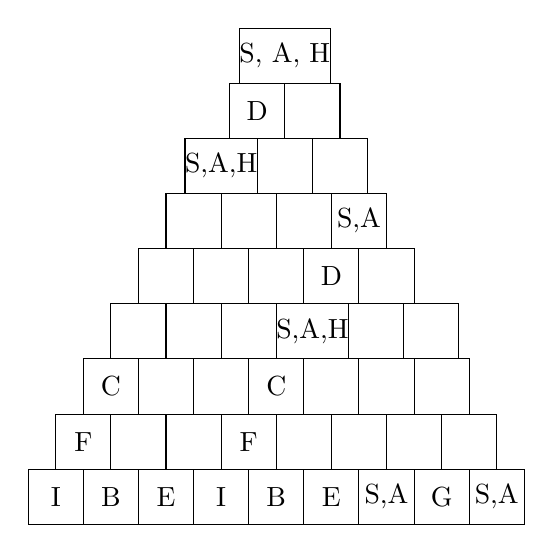
\begin{tikzpicture}[
                node distance = 0pt,
                every node/.style = {draw, minimum size=7mm, inner sep=0pt, outer sep=0pt}
            ]
                \node (n1)  {S, A, H};
                %
                \node (n11) [below left=of n1.south]    {D};
                \node (n12) [right=of n11]              {};
                %
                \node (n21) [below left=of n11.south]   {S,A,H};
                \node (n22) [right=of n21]              {};
                \node (n23) [right=of n22]              {};
                %
                \node (n31) [below left=of n21.south]   {};
                \node (n32) [right=of n31]              {};
                \node (n33) [right=of n32]              {};
                \node (n34) [right=of n33]              {S,A};
                %
                \node (n41) [below left=of n31.south]   {};
                \node (n42) [right=of n41]              {};
                \node (n43) [right=of n42]              {};
                \node (n44) [right=of n43]              {D};
                \node (n45) [right=of n44]              {};

                %
                \node (n51) [below left=of n41.south]   {};
                \node (n52) [right=of n51]              {};
                \node (n53) [right=of n52]              {};
                \node (n54) [right=of n53]              {S,A,H};
                \node (n55) [right=of n54]              {};
                \node (n56) [right=of n55]              {};
                %
                \node (n61) [below left=of n51.south]   {C};
                \node (n62) [right=of n61]              {};
                \node (n63) [right=of n62]              {};
                \node (n64) [right=of n63]              {C};
                \node (n65) [right=of n64]              {};
                \node (n66) [right=of n65]              {};
                \node (n67) [right=of n66]              {};
                %
                \node (n71) [below left=of n61.south]   {F};
                \node (n72) [right=of n71]              {};
                \node (n73) [right=of n72]              {};
                \node (n74) [right=of n73]              {F};
                \node (n75) [right=of n74]              {};
                \node (n76) [right=of n75]              {};
                \node (n77) [right=of n76]              {};
                \node (n78) [right=of n77]              {};
                %
                \node (n81) [below left=of n71.south]   {I};
                \node (n82) [right=of n81]              {B};
                \node (n83) [right=of n82]              {E};
                \node (n84) [right=of n83]              {I};
                \node (n85) [right=of n84]              {B};
                \node (n86) [right=of n85]              {E};
                \node (n87) [right=of n86]              {S,A};
                \node (n88) [right=of n87]              {G};
                \node (n89) [right=of n88]              {S,A};

            \end{tikzpicture}
        \end{minipage}
        \caption{CYK-Parser für mehrdeutige Grammatik}
        \label{fig:figure10}
    \end{figure}

    Eine wichtige Anmerkung zu der hier gezeigten Grammatik ist, dass zur besseren Darstellung der Tabelle,
    die Nichtterminale $ausdruck$ und $bedingung$ hier als Terminalsymbole in der Grammatik aufgeführt sind.
    Wie an diesem Ergebnis zu erkennen ist, findet der CYK-Parser hier alle mögliche Ableitungen für das gegebene Wort.
    Der Parser kann nun anhand festgelegter Regeln eindeutig entscheiden,
    welche dieser Ableitungen die richtige ist.


    \section{Fazit}\label{sec:zusammenfassung}

    Abschließend lässt sich festhalten, dass Mehrdeutigkeiten in Grammatiken von Programmiersprachen
    eine Herausforderung beim Parsen darstellen.
    Durch die Vermeidung von Mehrdeutigkeiten in der Sprache können einfachere und effizientere Parser verwendet werden.
    Neuere Programmiersprachen wie Swift\cite{apple2024swift} oder C\# vermeiden Mehrdeutigkeiten
    und können daher effizienter, beispielsweise mit einfachen Lookahead-Parsern, geparst werden.
    Wenn zudem vermieden werden kann, dass Mehrdeutigkeiten an den Entwickler weitergegeben werden,
    erleichtert es zusätzlich die Entwicklung in der jeweiligen Sprache.
    Auf der anderen Seite kann die Vermeidung von Mehrdeutigkeiten zu Boilerplate-Code führen.
    Die Tatsache, dass viele gängige Programmiersprachen wie C, Java oder Python Mehrdeutigkeiten aufweisen,
    zeigt, dass Mehrdeutigkeiten in Programmiersprachen praxistauglich sind.
    Ein weiteres Beispiel für die Eignung von mehrdeutiger Sprache im Programmieren ist AppleScript\cite{apple2016script},
    welches eine Syntax ähnlich der natürlichen Sprache besitzt
    und damit besonders einsteigerfreundlich ist.
    Die Tatsache aber, dass mehrdeutiger Code das Programmieren erschweren kann
    und dass Parser für mehrdeutige Sprachen weniger effizient sind,
    zeigt, dass bei der Konzeption einer neuen Programmiersprache
    darauf geachtet werden sollte, Mehrdeutigkeiten grundsätzlich zu vermeiden
    und nicht an den Entwickler weiterzugeben.

%
% ---- Bibliography ----
%
% BibTeX users should specify bibliography style 'splncs04'.
% References will then be sorted and formatted in the correct style.
%


    %\nocite{*}
    \bibliographystyle{splncs04}
    \bibliography{refs}
\end{document}
